% vim: foldmethod=marker: 
\documentclass[11pt]{standalone}

\usepackage[utf8]{inputenc}
\usepackage[T1]{fontenc}    


\usepackage{tikz}
\usetikzlibrary{arrows}

\begin{document}
    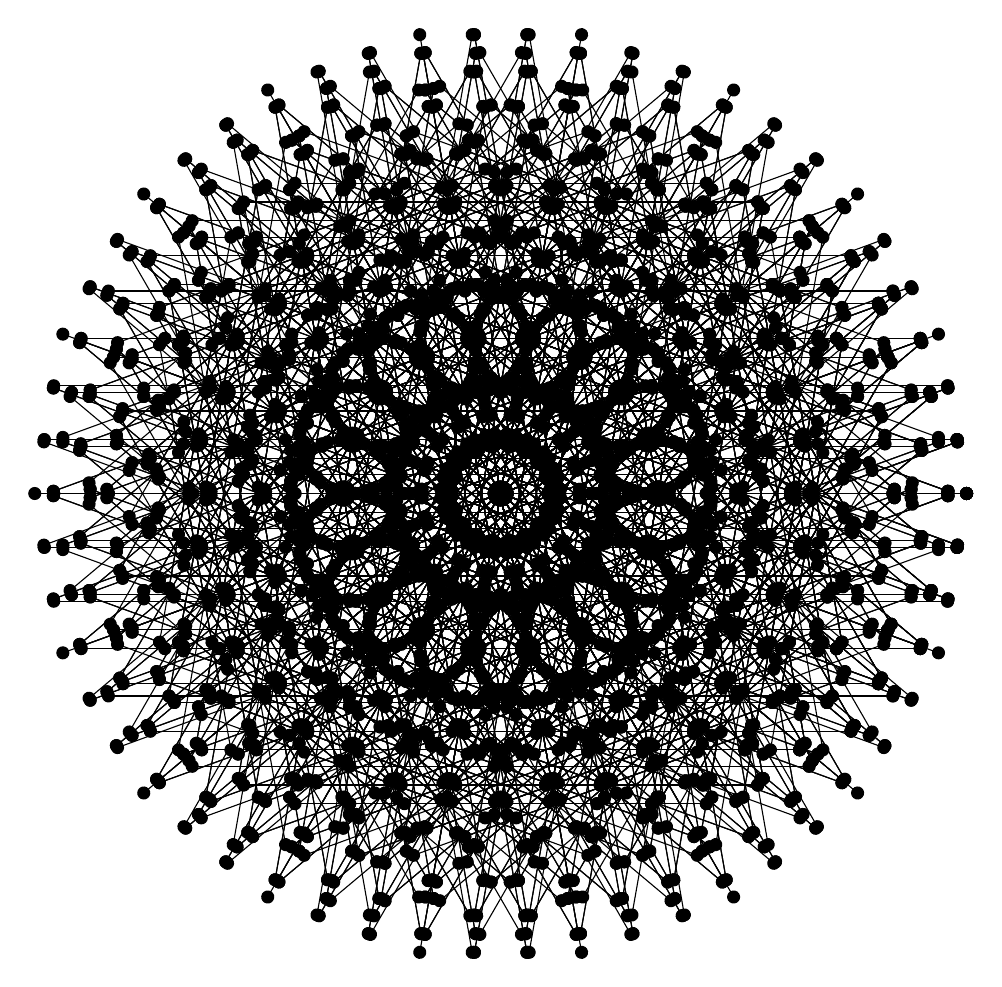
\begin{tikzpicture}
        \def\r{2}
        
        \foreach \xa in {0,20,...,360}{
            \draw[-*, color=black] (0,0) -- (\xa:\r);

            \foreach \xb in {0,20,...,360}{
                \draw[-*,color=black] (\xa:\r) -- + (\xb:\r) coordinate (fov); 

                \foreach \xc in {0,20,...,360}{
                    \draw[-*,color=black] (fov) -- + (\xc:\r); 

                }
            }
        }
        
    \end{tikzpicture}
\end{document}


